\subsection{One Family of Matrix-State Mixers}

\begin{frame}{One Family, One Table}
    Linear attention, gated recurrences, state-space models and the delta rule are all rules for updating a matrix state, read out as $o_t=S_tq_t$.
    \vspace{0.3em}
    \begin{center}
    \small
    \renewcommand{\arraystretch}{1.25}
    \begin{adjustbox}{max width=\linewidth}\begin{tabular}{lll}
        \toprule
        \textbf{Model} & \textbf{State update} & \textbf{What it adds} \\
        \midrule
        Linear attention & $S_t=S_{t-1}+v_tk_t^\top$ & nothing: write only \\
        RetNet & $S_t=\gamma\, S_{t-1}+v_tk_t^\top$ & fixed decay \\
        Mamba-2 & $S_t=\gamma_t\, S_{t-1}+v_tk_t^\top$ & input-dependent decay \\
        GLA & $S_t=S_{t-1}\mathrm{Diag}(\alpha_t)+v_tk_t^\top$ & per-channel decay \\
        DeltaNet & $S_t=S_{t-1}(I-\beta_tk_tk_t^\top)+\beta_tv_tk_t^\top$ & targeted overwrite \\
        \rowcolor{KAUSTcyan!12} Gated DeltaNet & $S_t=S_{t-1}\,\alpha_t(I-\beta_tk_tk_t^\top)+\beta_tv_tk_t^\top$ & decay and overwrite \\
        \bottomrule
    \end{tabular}\end{adjustbox}
    \end{center}
    \vspace{0.2em}
    \begin{itemize}
        \item Each transition stays \textbf{diagonal plus low-rank}. That structure is what keeps chunkwise training possible.
    \end{itemize}
    \src{After Yang et al., \href{https://arxiv.org/abs/2406.06484}{arXiv:2406.06484}, Table 2, and Yang, Kautz, Hatamizadeh, \href{https://arxiv.org/abs/2412.06464}{arXiv:2412.06464}.}
\end{frame}

\begin{frame}{Mamba-3 (2026): Designed for Inference First}
    \begin{columns}[T,onlytextwidth]
        \column{0.5\textwidth}
        \begin{itemize}\itemsep0.25em
            \item \textbf{Better discretisation.} A trapezoidal rule replaces the separate conv layer.
            \item \textbf{Complex-valued state.} The state can \emph{rotate}, which scalar decay cannot. It acts as a data-dependent RoPE.
            \item \textbf{MIMO.} More compute per decode step, same state size.
        \end{itemize}
        \vspace{0.3em}
        \footnotesize
        \begin{adjustbox}{max width=\linewidth}\begin{tabular}{lcc}
            \toprule
            \textbf{At 1.5B} & \textbf{Mamba-3} & \textbf{Mamba-2} \\
            \midrule
            Perplexity & 10.24 & 10.47 \\
            Parity task & 100\% & 0.9\% \\
            \bottomrule
        \end{tabular}\end{adjustbox}
        \column{0.48\textwidth}
        \centering
        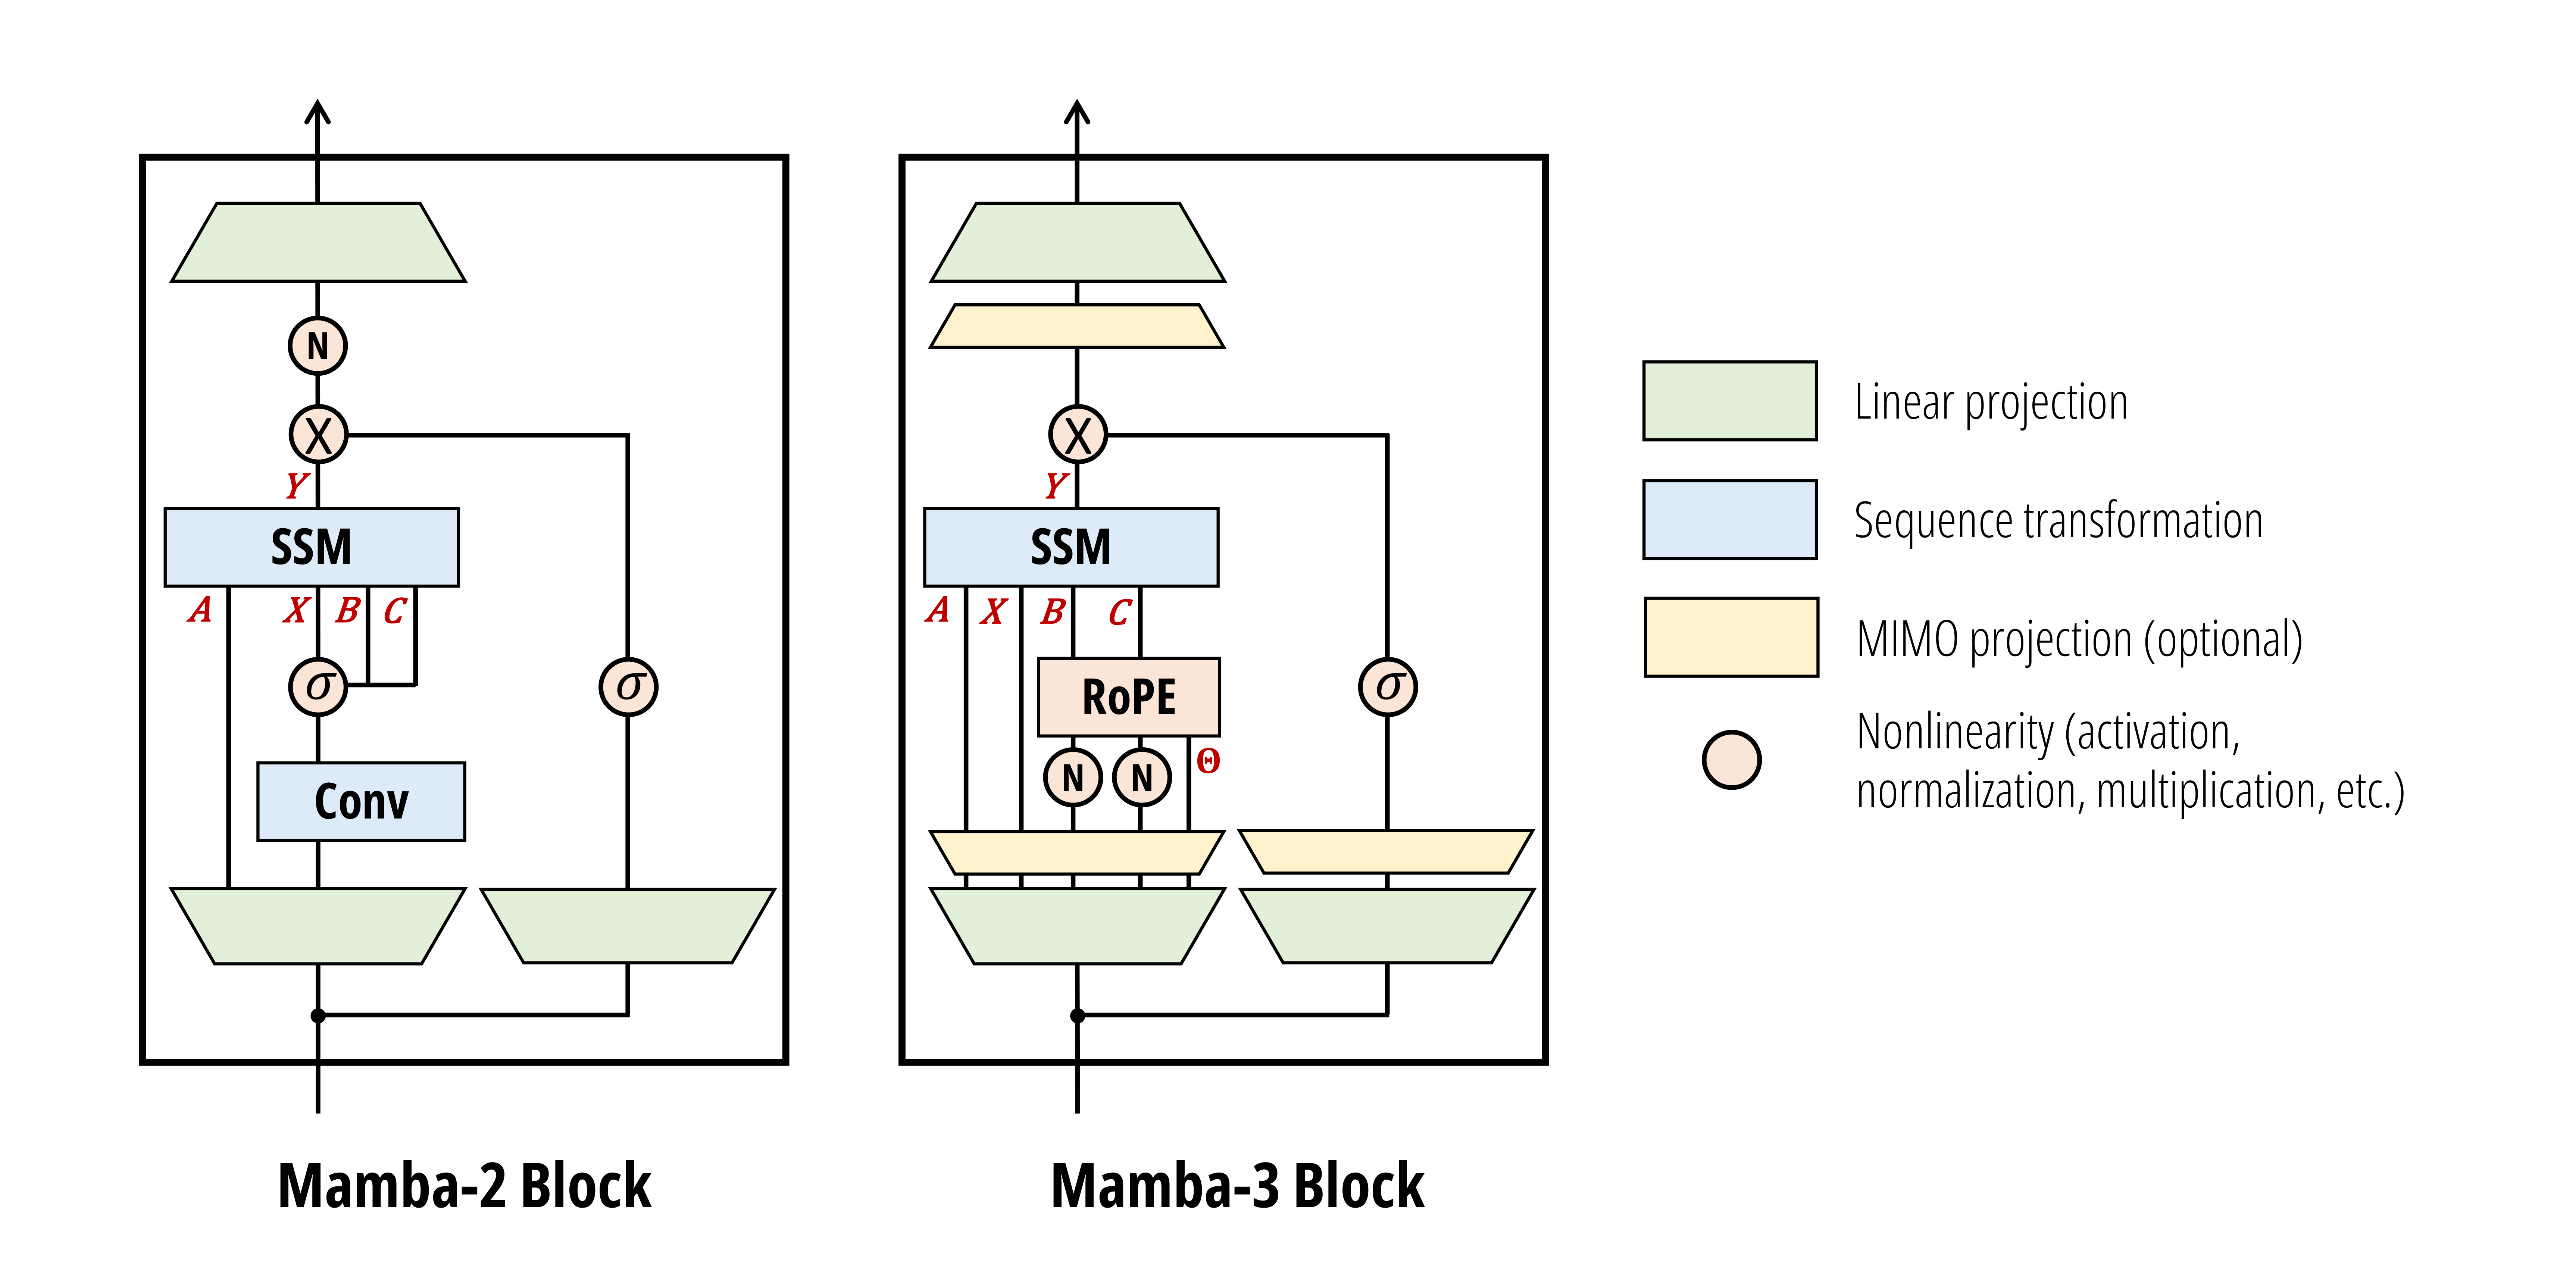
\includegraphics[width=\linewidth,height=0.5\textheight,keepaspectratio]{images/next-gen-architectures/mamba3_arch.png}
    \end{columns}
    \vspace{0.2em}
    \caveat{Results stop at 1.5B parameters. No shipped production model used Mamba-3 as of October 2026.}
    \src{Lahoti et al., ``Mamba-3: Improved Sequence Modeling using State Space Principles,'' ICLR 2026, \href{https://arxiv.org/abs/2603.15569}{arXiv:2603.15569}. Figure: Goomba Lab blog, ``Mamba-3 Part 1'' (2026).}
\end{frame}
